\section{Design og Implementering}
Denne section beskriver design og implementering af database delen som er lavet på baggrund af kravspecifikationen og systemarkitekturen.\\
Databasen er blevet opdelt i 2 dele som håndtere denne side. Databasen er opdelt i serveren og web-siden.
\begin{figure}[H]
\centering
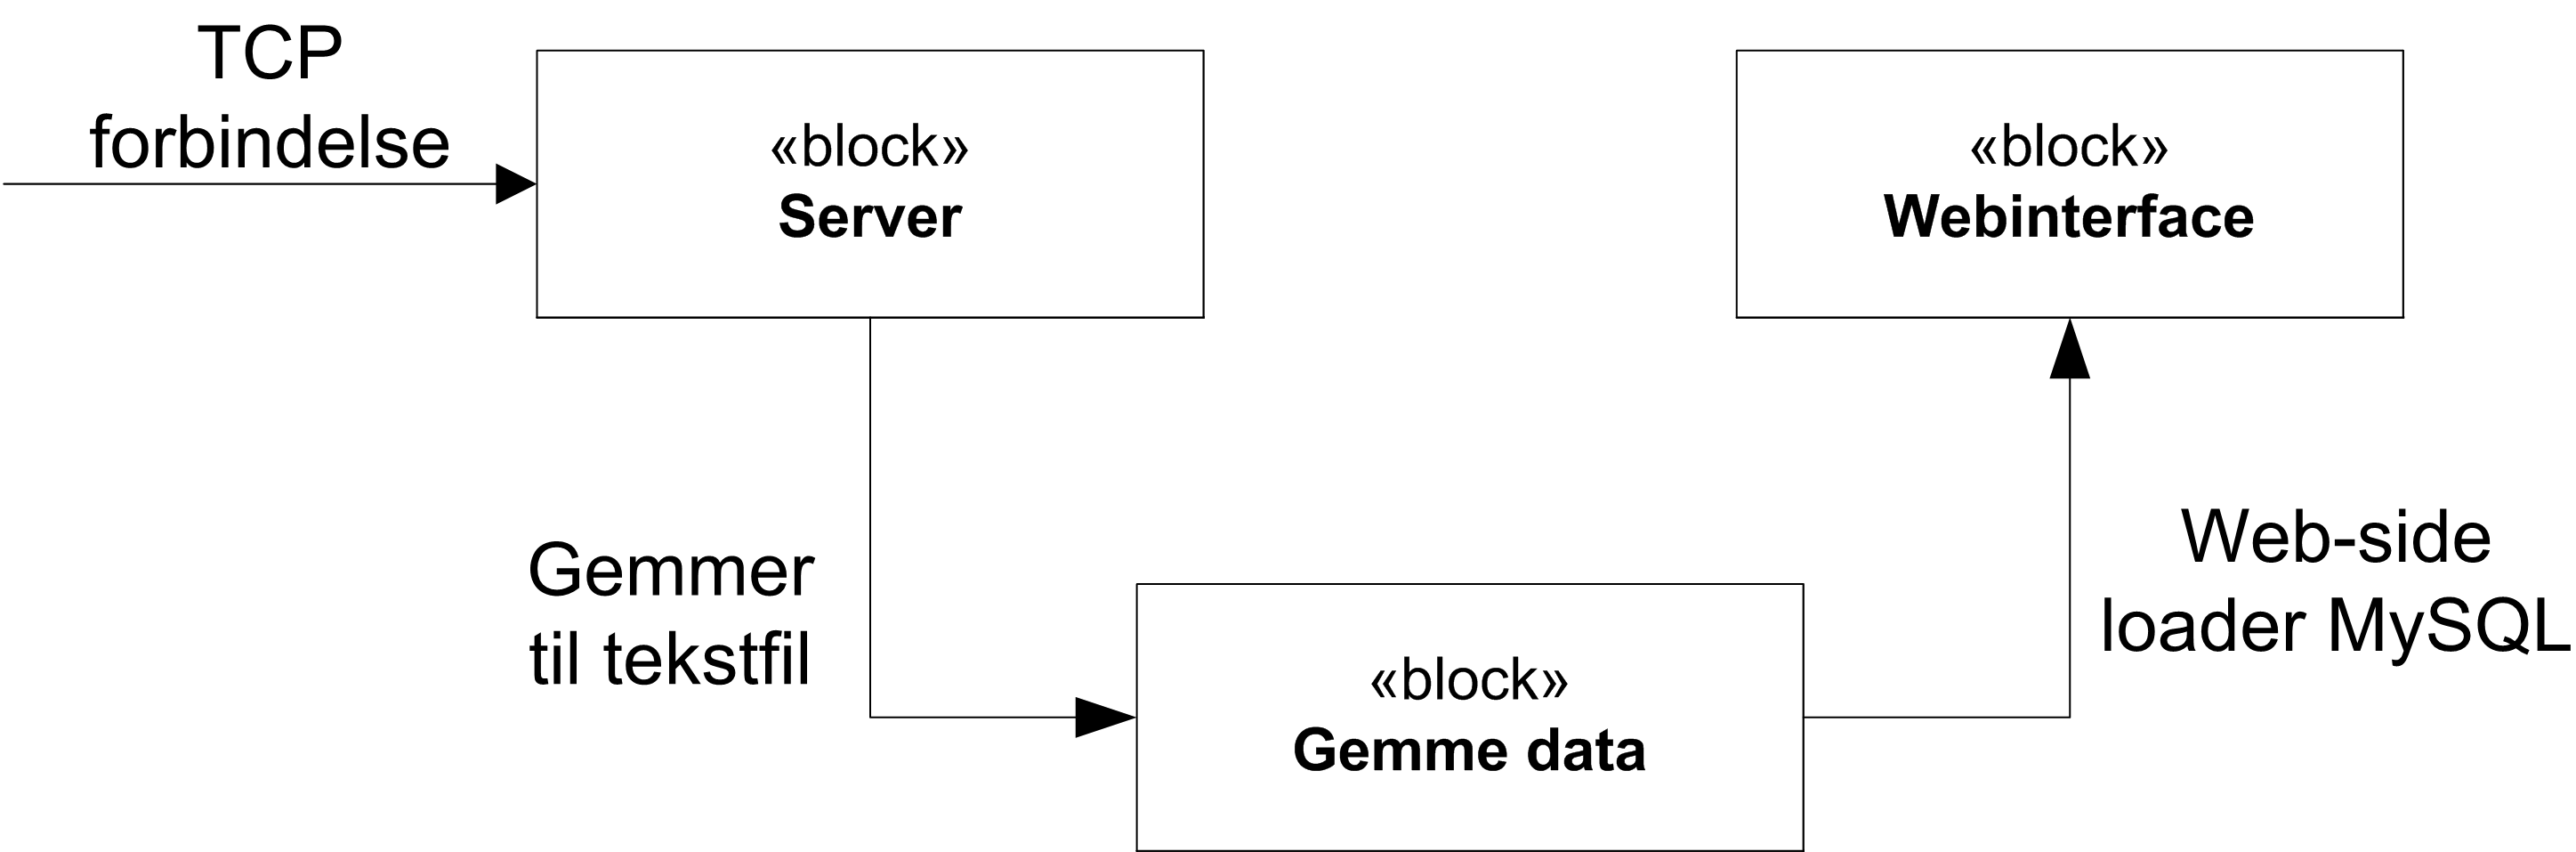
\includegraphics[width = 0.5\textwidth]{billeder/database_to_mysql}
\caption{Illustrere overordnet hvordan databasen fungere}
\label{fig:server_to_mysql}
\end{figure}

\subsection{Serveren}
Denne section besrkiver design og implementering af serveren.
Opbygningen af severen er gjort i klasser sådan at hver element i severen er implemnteret som en klasse se figur ??. Ud over dette benyttes der nogle hjælpeklasser.\\

Det gælder at når KI forsøger at kontakte databasen, tilsluttes denne via tcp som benytter sig af socket. Når tilslutningen er gjort kan der overføres data fra KI til databasen. Dataerne bliver gemt i mySQL databasen. I tilfælde af at der blvier problermer med at gemme, laves der en en tekst fil hvori dataerne bliver lagt og kan så forsøgt gemt af web siden.
\begin{figure}[H]
\centering
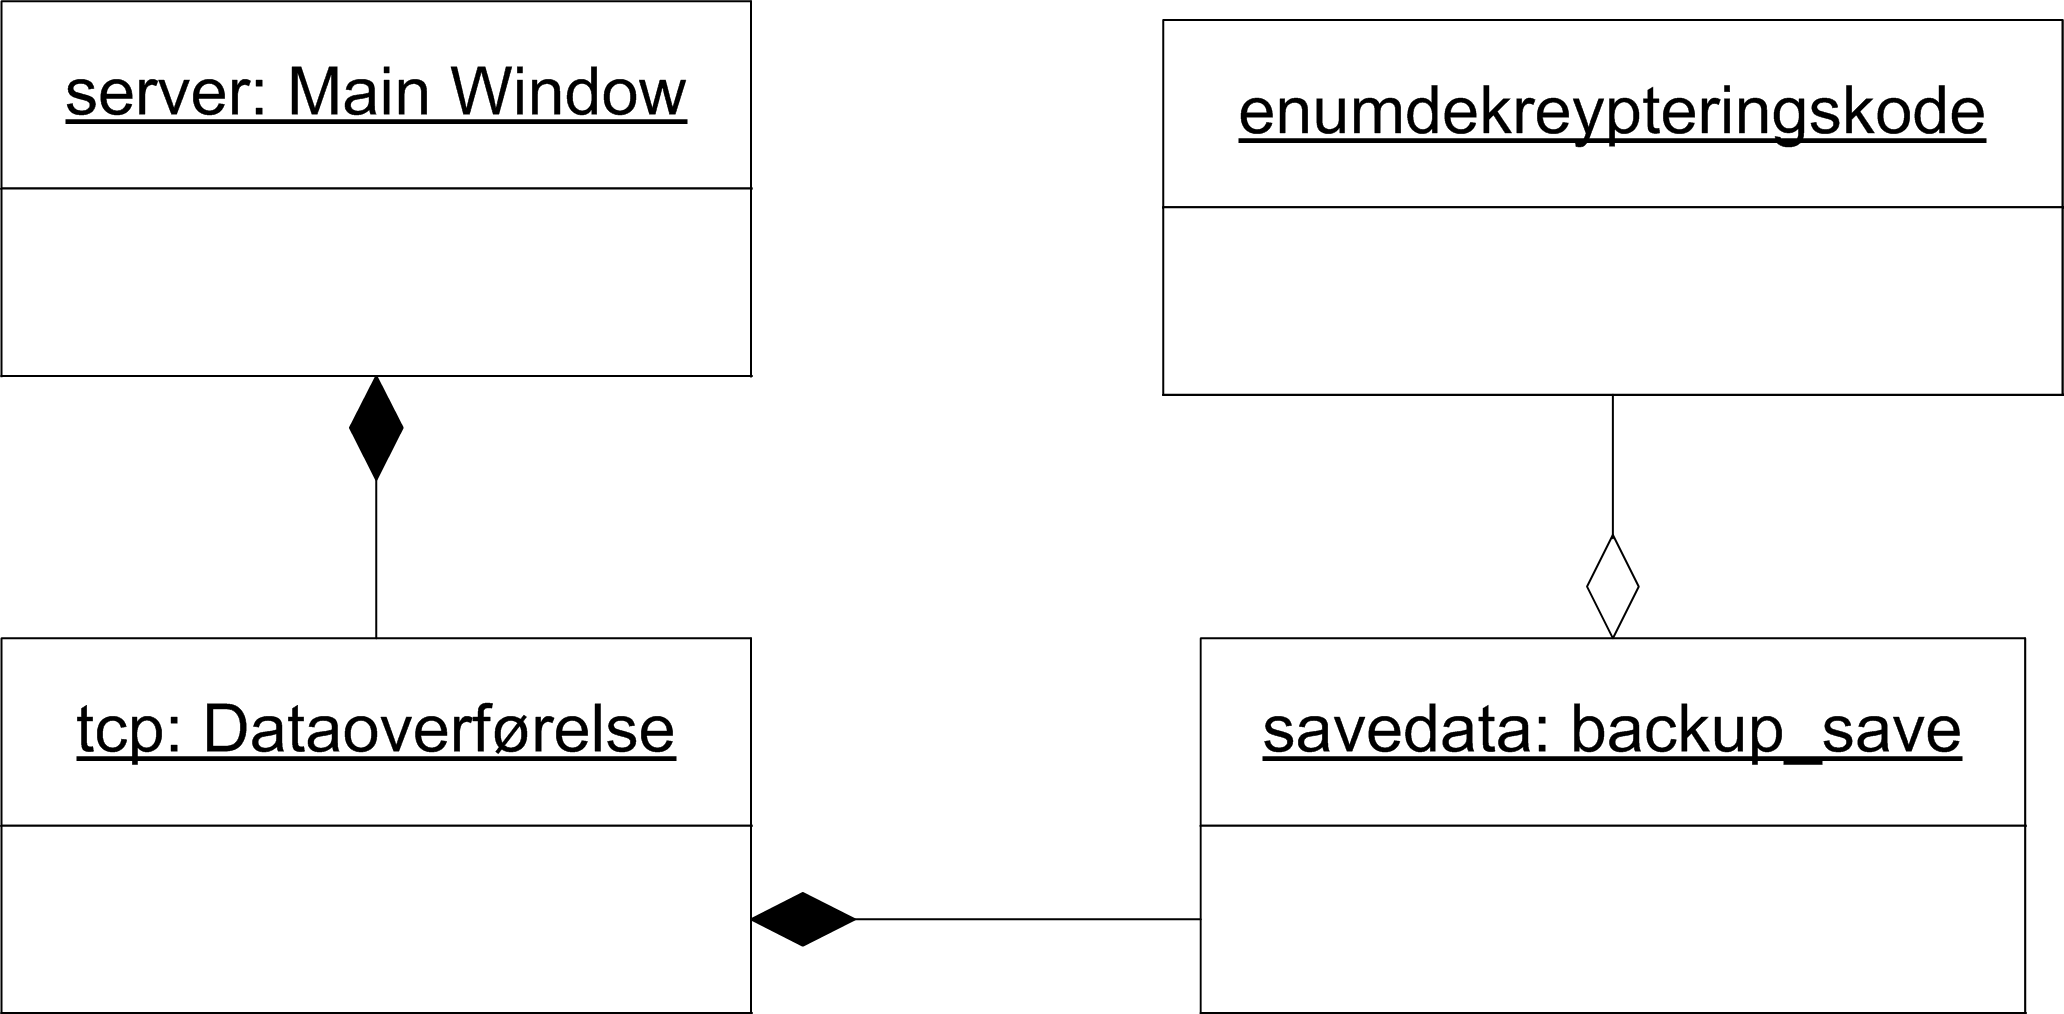
\includegraphics[width = 0.5\textwidth]{billeder/database_server}
\caption{Illustrere overordnet hvordan serveren fungere}
\label{fig:database_server}
\end{figure}
